\documentclass[10pt,a4paper]{article}
\usepackage[utf8]{inputenc}
\usepackage{graphicx}
\usepackage{tabularx}
\usepackage[normalem]{ulem}
\usepackage{fancyhdr}
\usepackage[left=2cm,right=2cm,top=2.0cm,bottom=2cm,headsep=1cm,a4paper]{geometry}
\pagestyle{fancy}
\renewcommand{\headrulewidth}{0pt}
\setlength{\fboxsep}{1.5em}
\setlength{\headheight}{5em}
\linespread{1.8}
\usepackage{xskak,chessboard}

\rhead{\huge \fbox{\parbox{3.5cm}{Score}}}
\begin{document}
\centering
\Huge
MARVEL Pub Quiz
\vspace{2cm}

\LARGE
Team Name: \underline{\hphantom{XXXXXXXXXXXXXXXXXXXXXXXXXX}}

\vspace{3cm}

\LARGE
\begin{tabular}{ll}
\hline
Round & Score \\
\hline
Switzerland & \\
``Marvel'' & \\
Design and Discovery of Novel Materials & \\
Changing things up & \\
Numbers & \\
Pictures: Surmise by size & \\
Puzzles: Connect Four & \\
TOTAL \\
\hline
\end{tabular}
\thispagestyle{empty}
\Huge
\newpage
\begin{center}
\Huge
Round 1: Switzerland
\end{center}
\large
\Huge
\begin{enumerate}
\item
\item
\item
\item
\item
\item
\item
\item
\end{enumerate}

\newpage
\begin{center}
\Huge
Round 2: ``Marvel''
\end{center}
\large
\Huge
\begin{enumerate}
\item
\item
\item
\item
\item
\item
\item
\item
\end{enumerate}

\newpage
\begin{center}
\Huge
Round 3: Design and Discovery of Novel Materials
\end{center}
\large
\Huge
\begin{enumerate}
\item
\item
\item
\item
\item
\item
\item
\item
\end{enumerate}

\newpage
\begin{center}
\Huge
Round 4: Changing things up
\end{center}
\large
\Huge
\begin{enumerate}
\item
\item
\item
\item
\item
\item
\item
\item
\end{enumerate}

\newpage
\begin{center}
\Huge
Round 5: Numbers
\end{center}
\large
The answers to the questions in this round are the numbers 1 to 8, without repeat

\Huge
\begin{enumerate}
\item
\item
\item
\item
\item
\item
\item
\item
\end{enumerate}

\newpage
\begin{center}
\Huge
Pictures: Surmise by size
\end{center}
\large
Each of the following maps show the world, but with each country resized based on a different statistic. Identify the statistic for each map. The country with the largest value has been labelled. Use the QR code to see the maps in greater detail.

\begin{center}

\includegraphics[width=0.2\textwidth]{maps/qr.png}
\end{center}

\linespread{1.2}

\begin{center}
\LARGE
\begin{tabularx}{0.75\textwidth}{XX}
    1. & 2. \\
    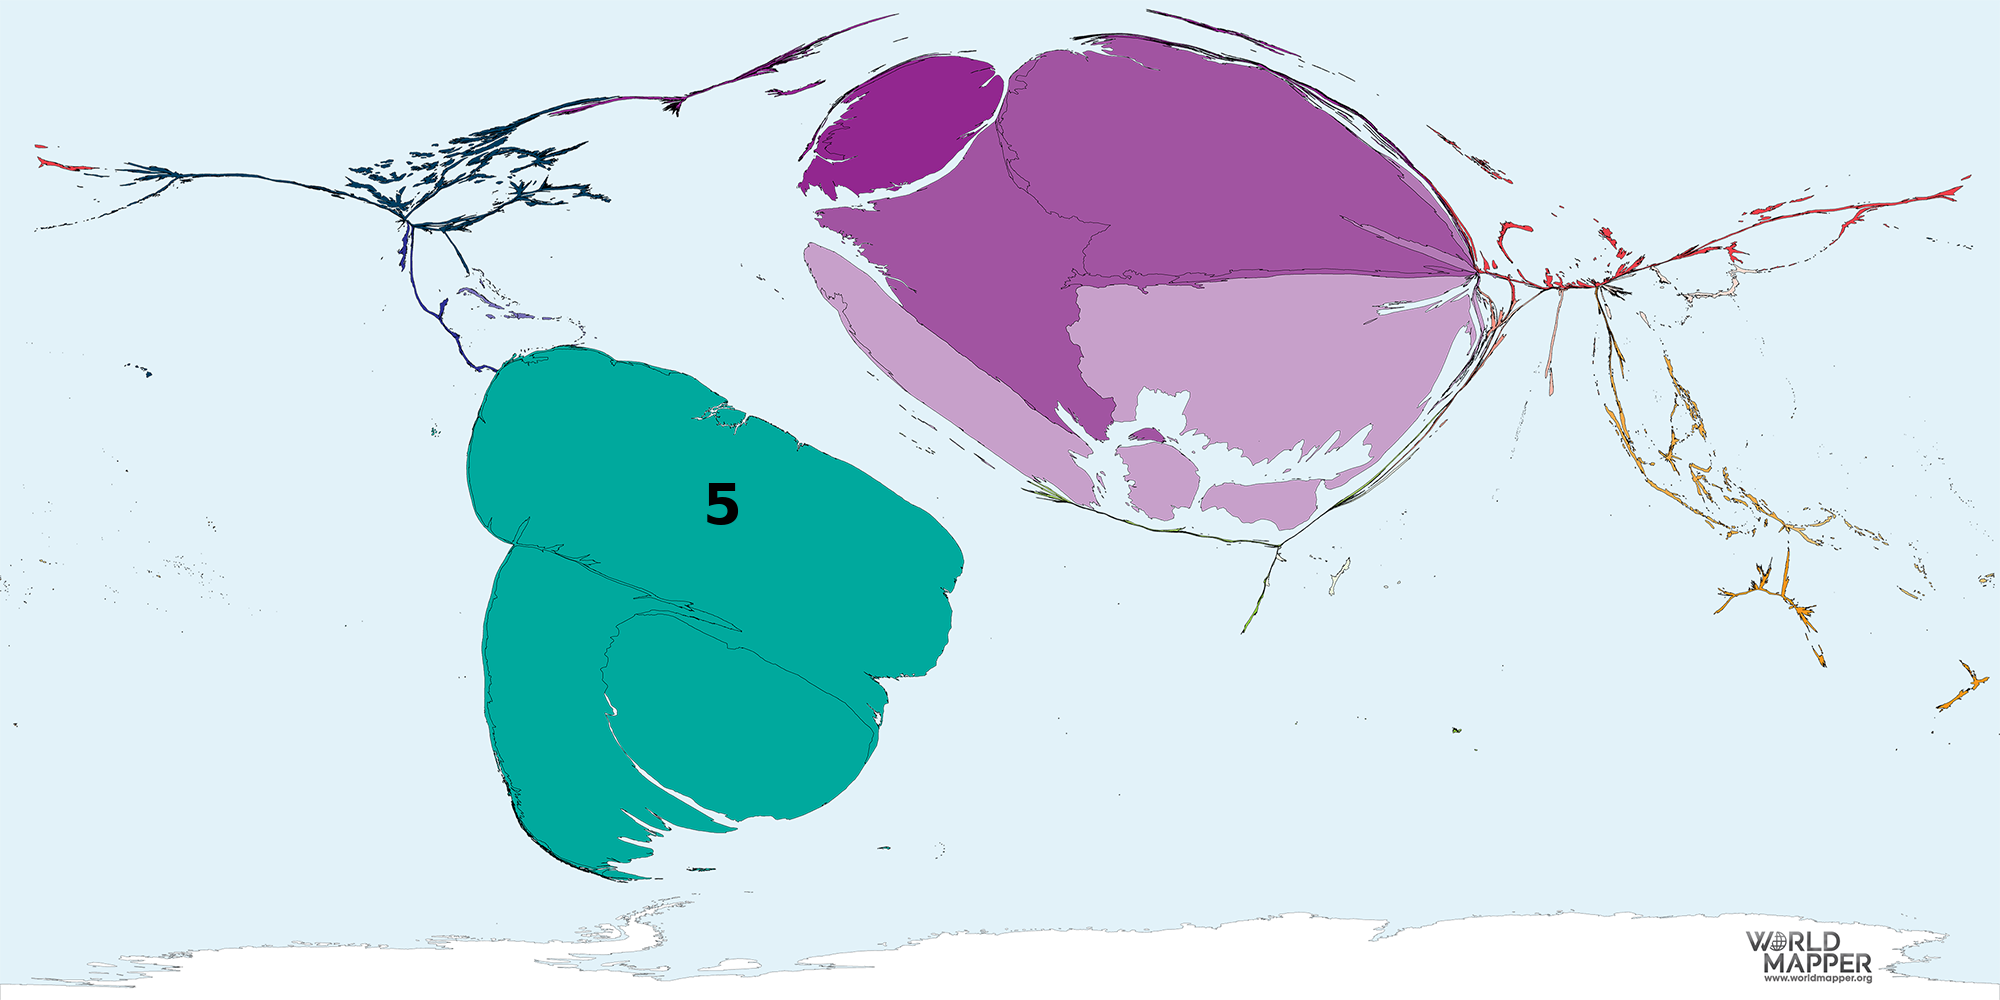
\includegraphics[width=0.35\textwidth]{maps/picture_1.png} &
    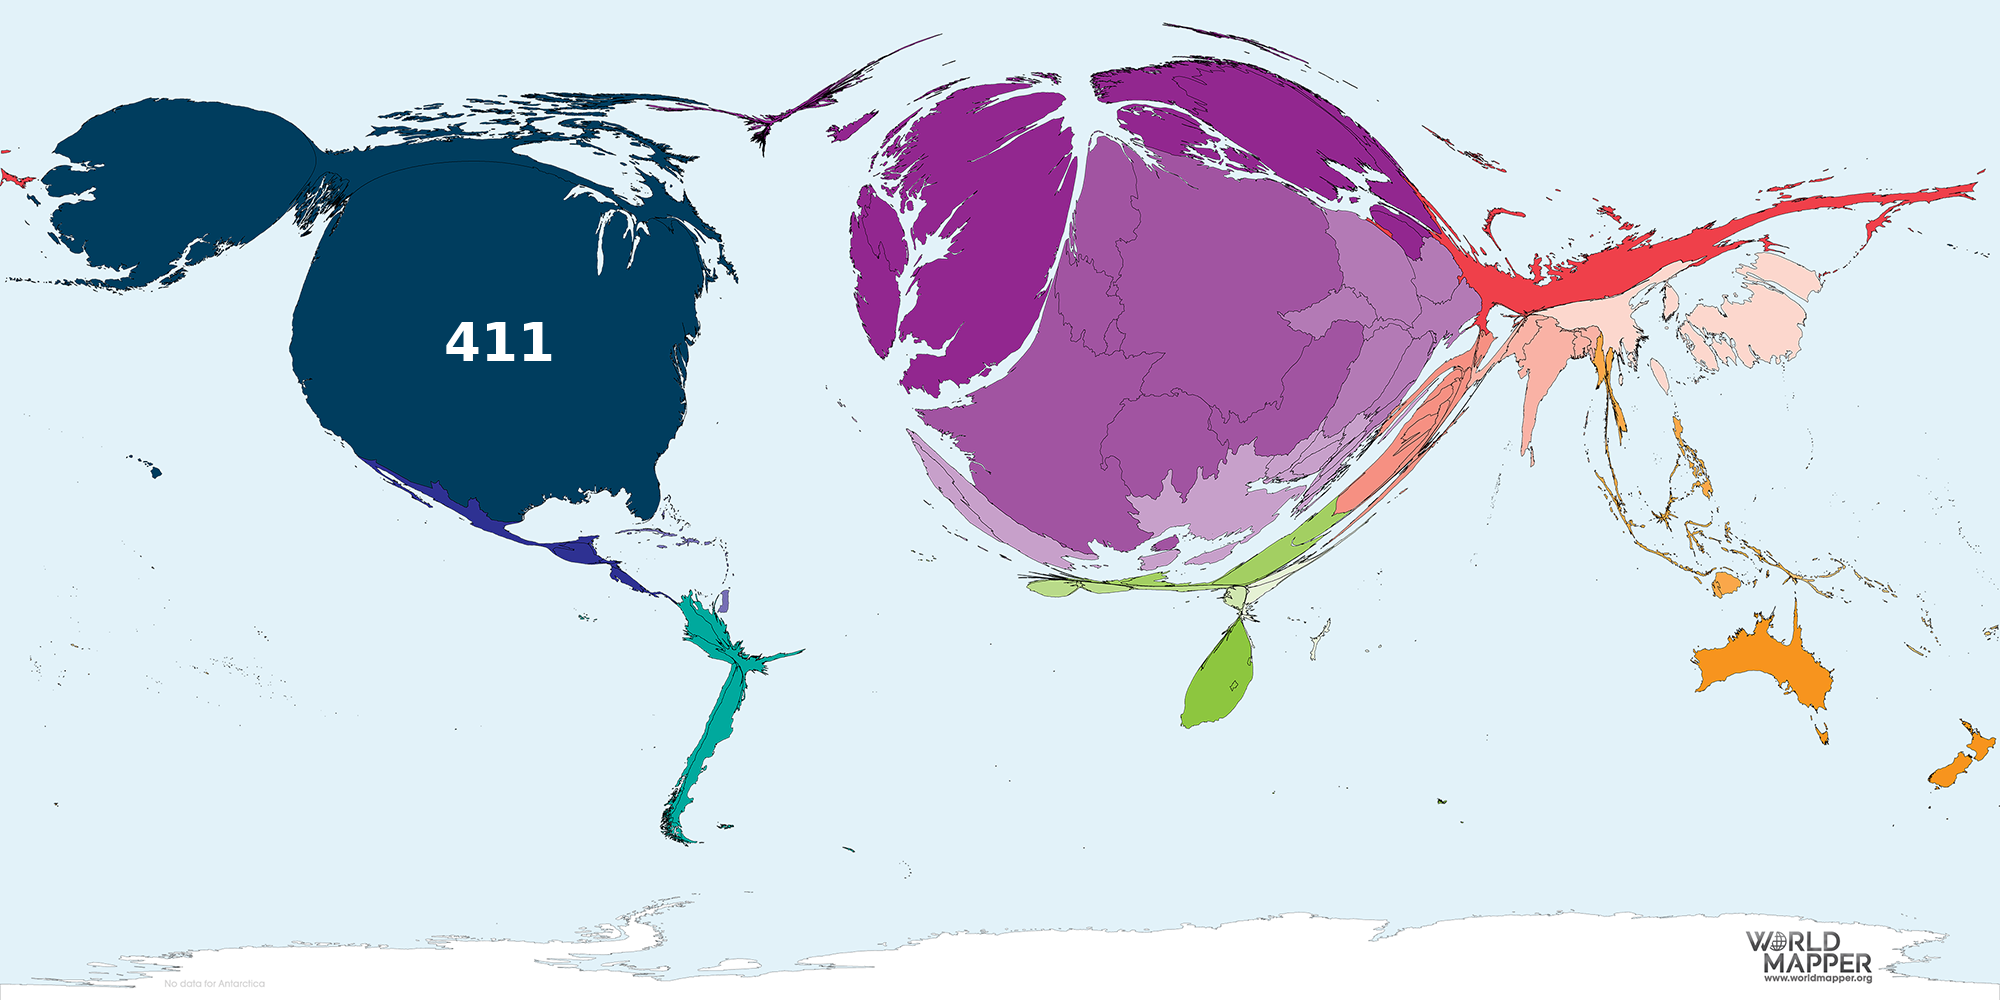
\includegraphics[width=0.35\textwidth]{maps/picture_2.png} \\
    3. & 4. \\
    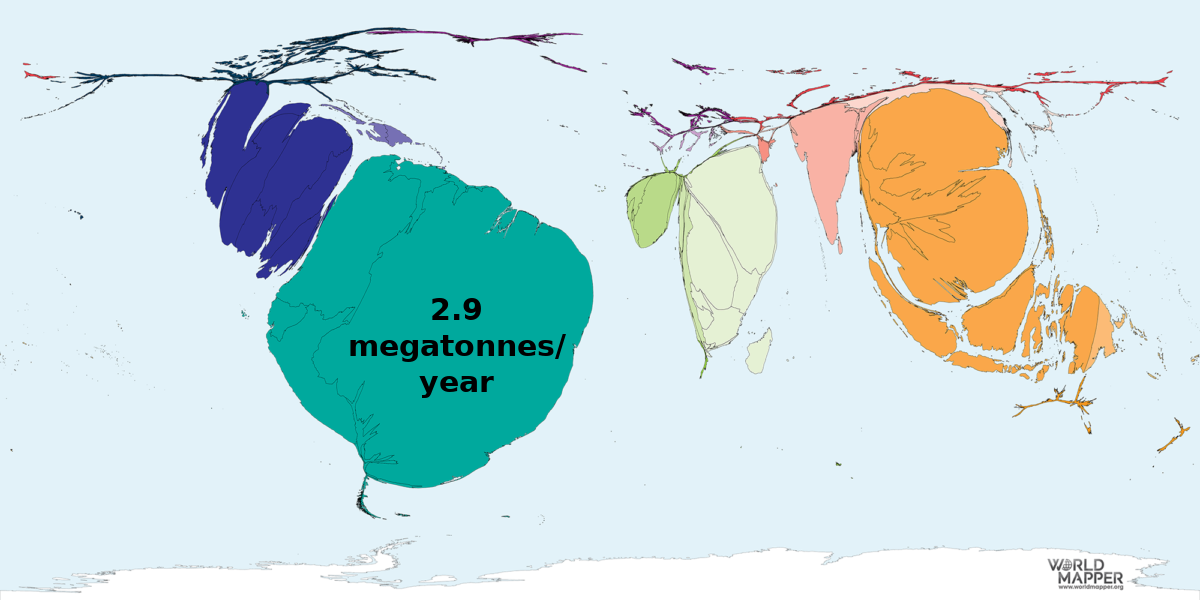
\includegraphics[width=0.35\textwidth]{maps/picture_3.png} &
    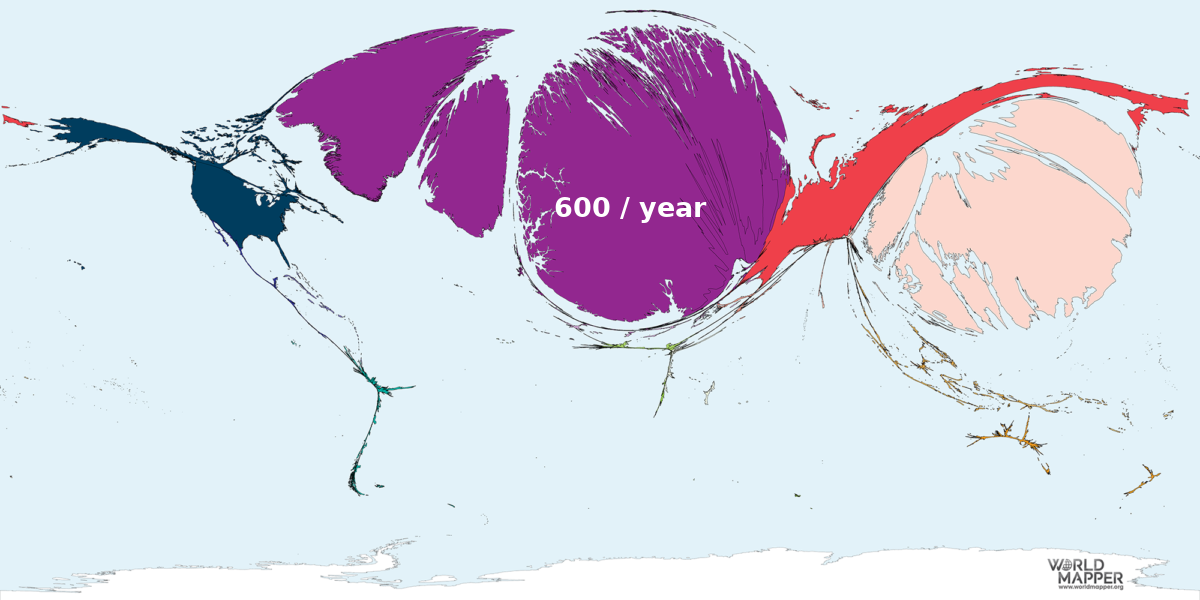
\includegraphics[width=0.35\textwidth]{maps/picture_4.png} \\
    5. & 6. \\
    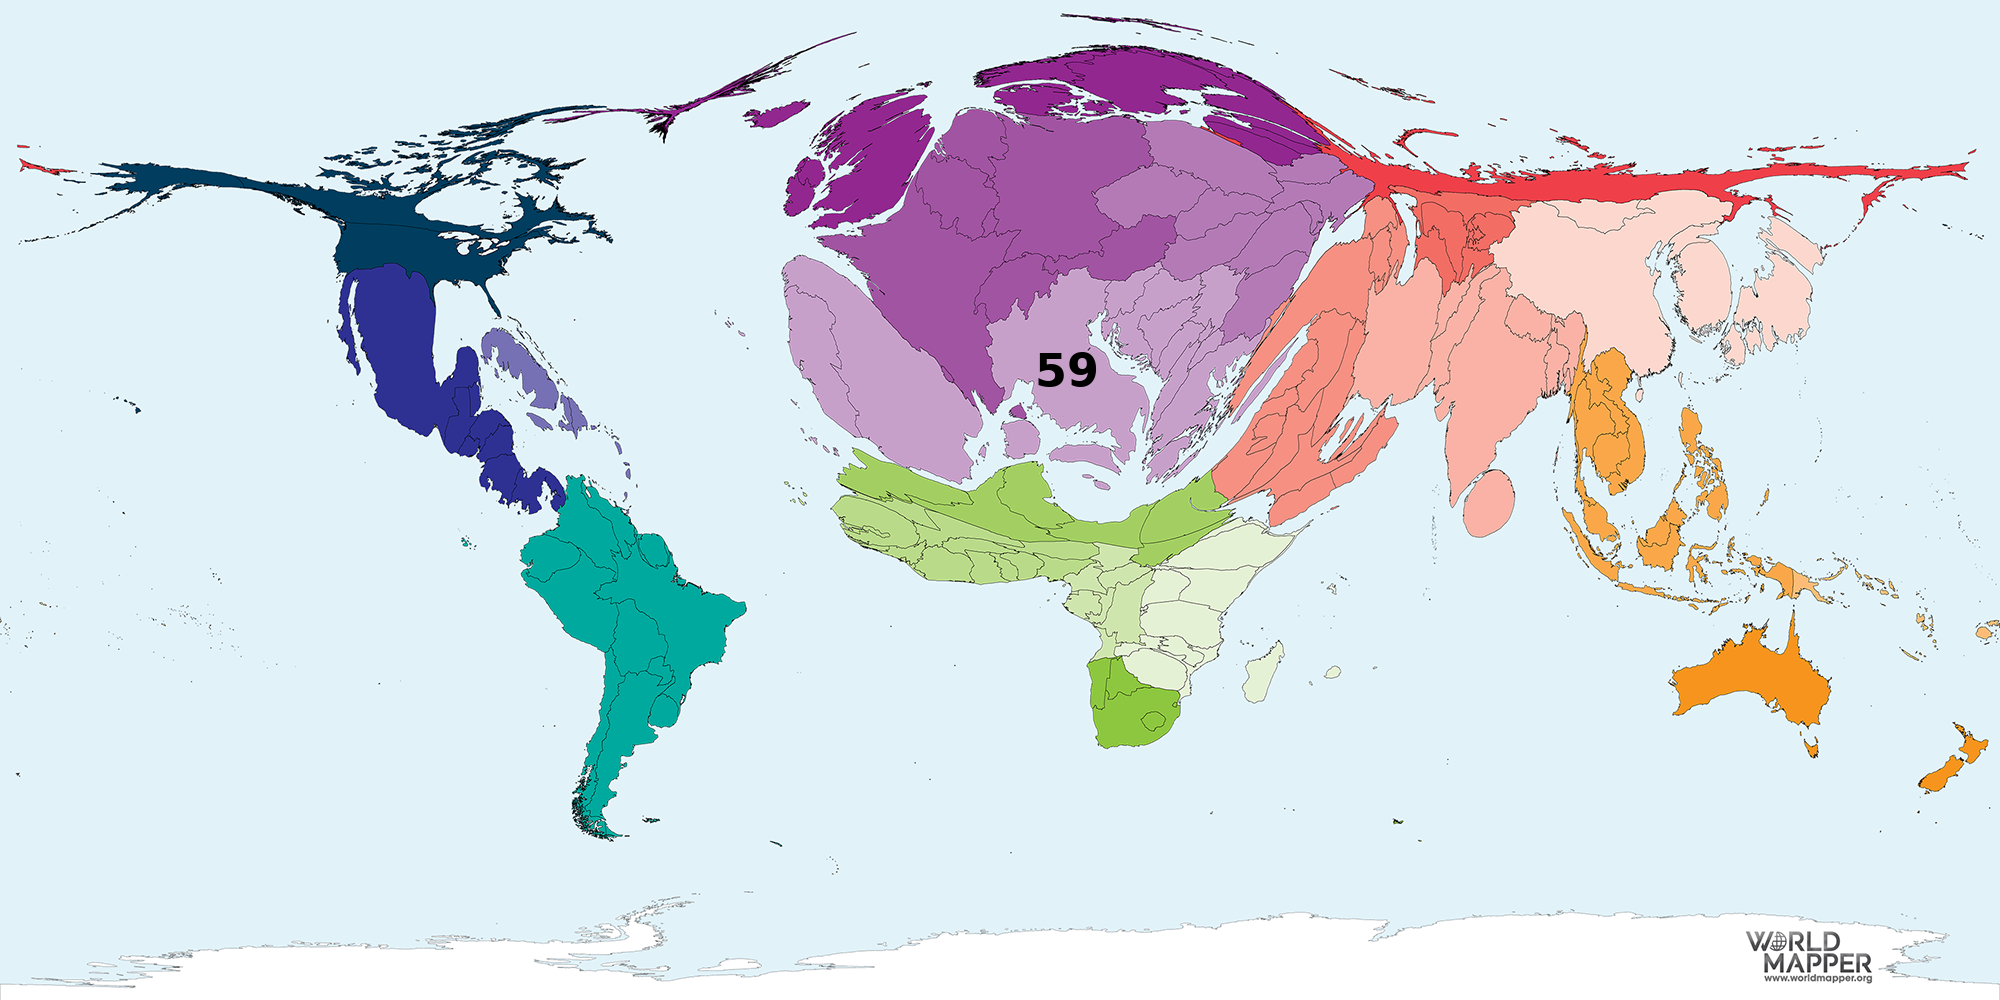
\includegraphics[width=0.35\textwidth]{maps/picture_5.png} &
    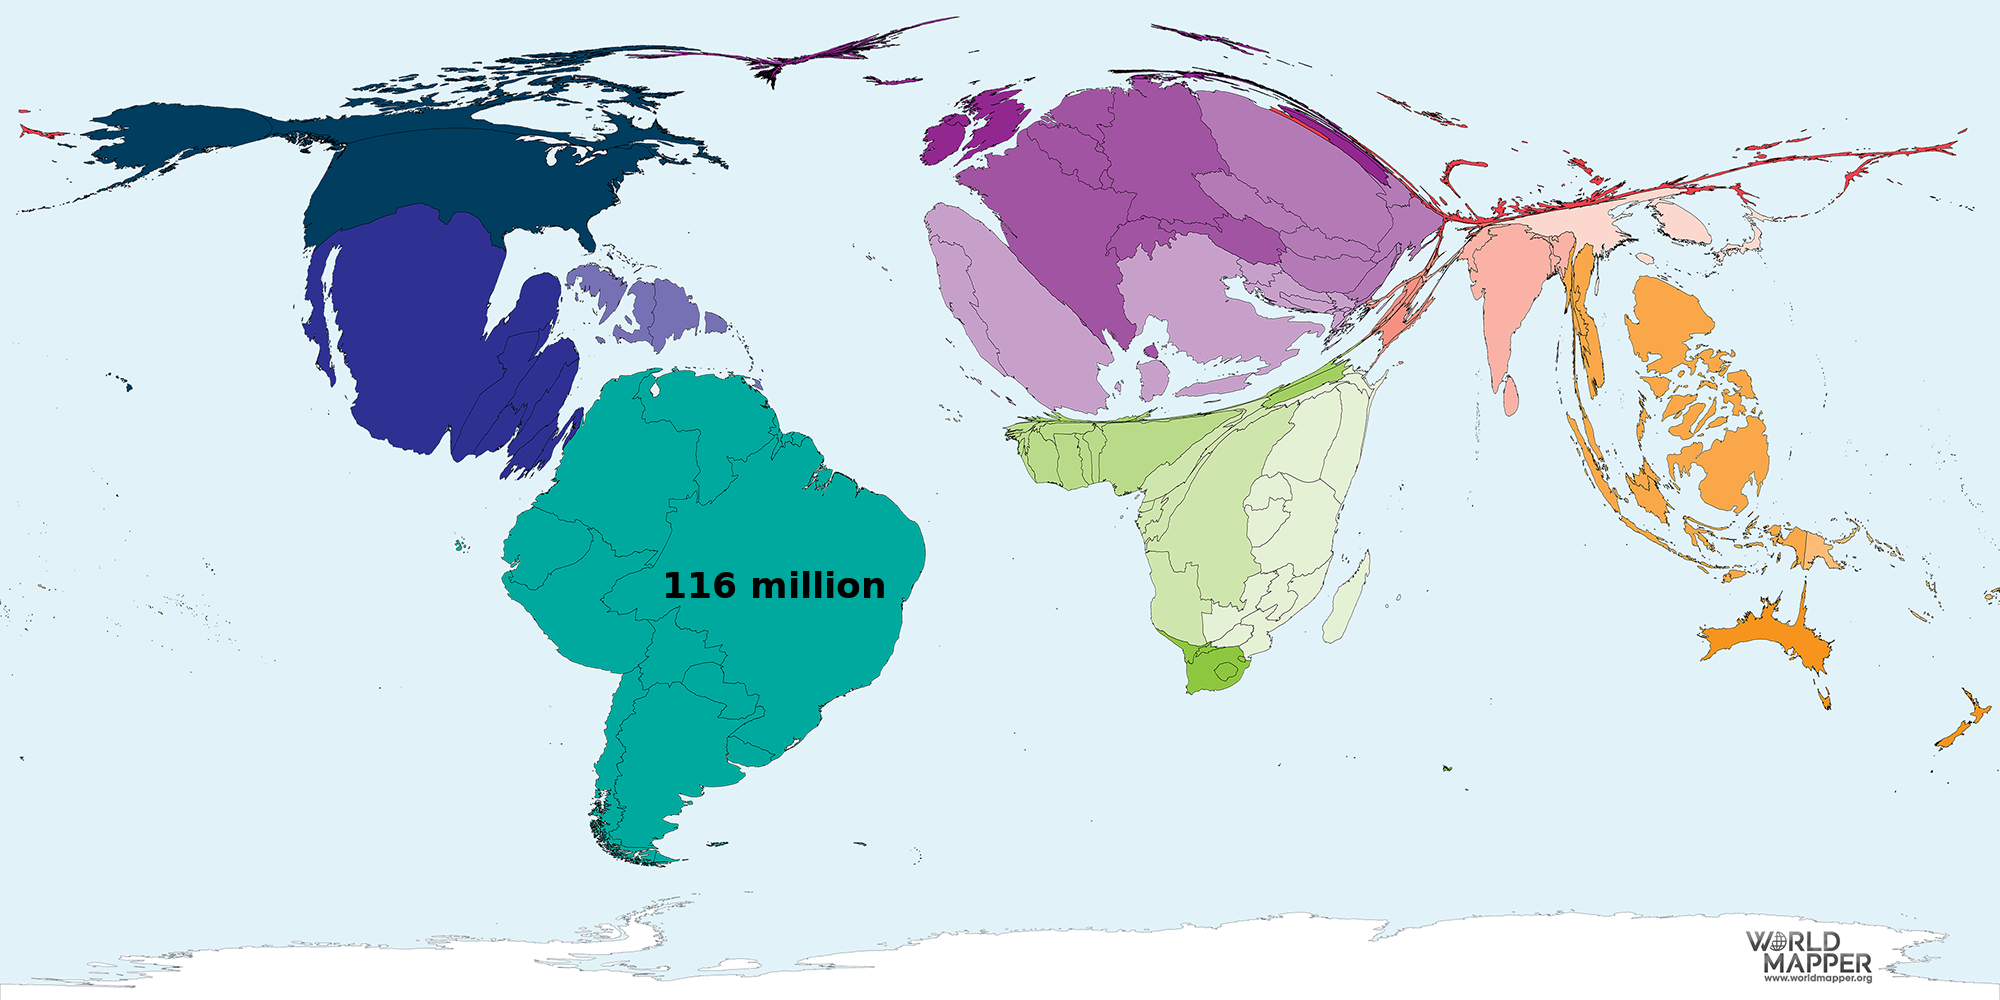
\includegraphics[width=0.35\textwidth]{maps/picture_6.png} \\
    7. & 8. \\
    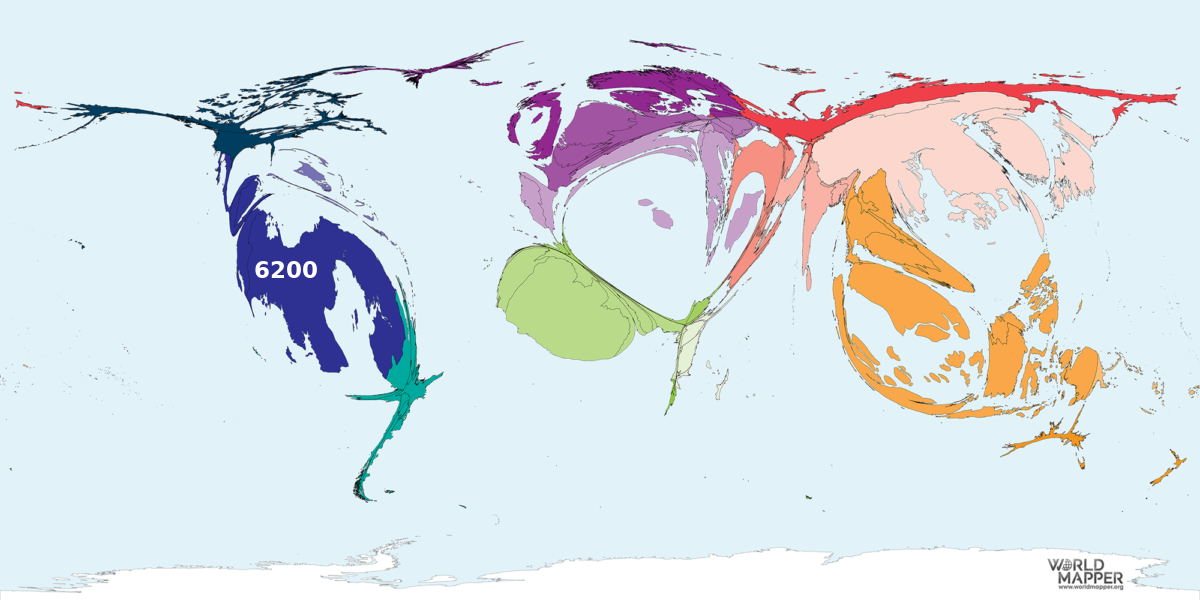
\includegraphics[width=0.35\textwidth]{maps/picture_7.png} &
    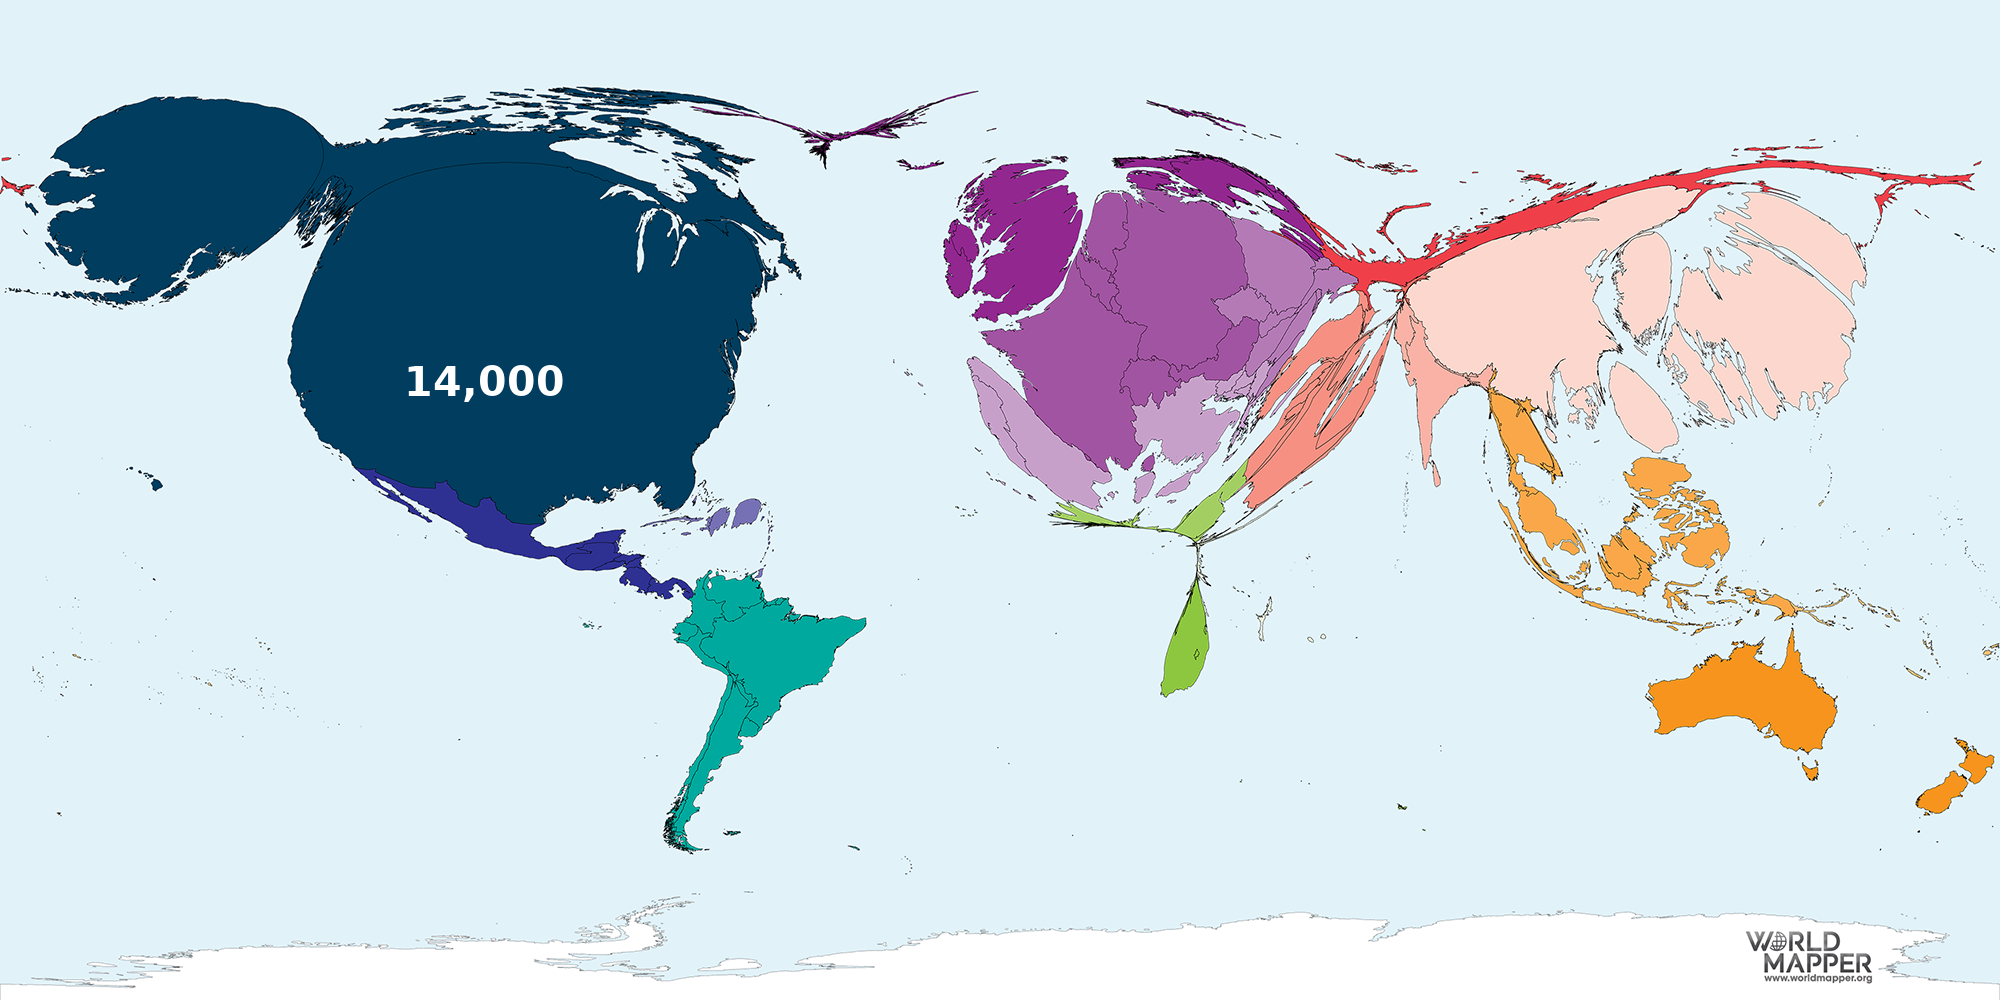
\includegraphics[width=0.35\textwidth]{maps/picture_8.png}
\end{tabularx}
\end{center}

\linespread{1.8}

\newpage
\begin{center}
\Huge
Puzzles: Connect Four
\end{center}
\large
For each puzzle, work out what connects the four items. Make your answers as specific as possible! Each puzzle is worth two points.

\large
\begin{enumerate}
\item \leavevmode \\
\begin{center}
    \begin{minipage}{0.6\textwidth}
        \textit{%
            sharp taste \\
            words set to music \\
            Solo character \\
            archenemy of Flash Gordon}%
    \end{minipage}
\end{center}

\item \leavevmode \\
\begin{center}
\setchessboard{boardfontsize=8pt, labelleft=false, labelbottom=false} % , labelfontsize=6pt
\newgame
\chessboard[setfen=4K3/8/8/8/8/8/8/8 w - - 0 0,showmover=False]
\chessboard[setfen=8/8/6K1/8/8/8/8/8 w - - 0 0,showmover=False]
\chessboard[setfen=8/8/8/8/8/8/4Q3/8 w - - 0 0,showmover=False]
\chessboard[setfen=8/8/8/8/8/2K5/8/8 w - - 0 0,showmover=False]
\end{center}
\item \leavevmode \\
\begin{center}
    \begin{minipage}{0.6\textwidth}
        \textit{%
            Test: objection and competition \\
            Found: deep and confuse \\
            Tract: extend and agreement \\
            Duct: goods and behaviour}%
    \end{minipage}
\end{center}

\item \leavevmode \\
\begin{center}
    \begin{minipage}{0.6\textwidth}
        \textit{%
            Somalia: very bad \\
            Syria: bad \\
            Philippines: average \\
            New Zealand: good}%
    \end{minipage}
\end{center}

\end{enumerate}

\end{document}